\documentclass[aps,onecolumn]{revtex4}
\usepackage{graphicx}
\usepackage{amssymb,amsfonts,amsmath,amsthm}
\usepackage{chemarr}
\usepackage{bm}
\usepackage{pslatex}
\usepackage{mathptmx}
\usepackage{xfrac}
\usepackage{xcolor}

\begin{document}

\section{Curvature of a revolution surface}

If we have
\begin{equation}
	r(t),\;\; z(t)
\end{equation}
then the mean curvature is equal to
\begin{equation}
	\mathcal{H} =  \dfrac{
		r \left(r''z'-r'z''\right)  - z' \left(r'^2+z'^2\right)
	}
	{
		2r\left(r'^2+z'^2\right)^{3/2}
	}
\end{equation}
We know use an intrinsic representation of the $(r,z)$ profile using the
angle $\phi$ and the variable $s$ so that
\begin{equation}
\left\lbrace
	\begin{array}{rcl}
	r' & = & \cos \phi\\
	z' & = & \sin \phi\\
	r'' & = & -\sin\phi \phi'\\
	z'' & = & \cos\phi  \phi'\\
	\end{array}
\right.
\end{equation}
and we get
\begin{equation}
	\mathcal{H} = -\frac{1}{2} \left(\phi'+\dfrac{\sin\phi}{r}\right)
\end{equation}

\section{Surface equation}
Since the capillary pressure is supporting the liquid
\begin{equation}
	\gamma \mathcal{H} = \rho g z
\end{equation}
or using the capillary length
\begin{equation}
	\lambda = \sqrt{\dfrac{\gamma}{\rho g}}
\end{equation}

\begin{equation}
	\mathcal{H} = \dfrac{z}{\lambda^2}
\end{equation}

\section{Bridge description}
\subsection{Polar Equation}
Let $\rho(\alpha)$ be a polar description of the lens, so that the bridge description in the $xy$ plane are
\begin{equation}
	\left\lbrace
	\begin{array}{rcl}
	x(\alpha) & = & \rho(\alpha)\sin\alpha\\
	y(\alpha) & = & h + R - \rho(\alpha)\cos\alpha\\
	\rho(0)   & = & R\\
	\rho'(0)  & = & 0\\
	\end{array}
	\right.
\end{equation}

\subsection{Contact Angle and Initial Profile Angle}
The   tangent vector is
\begin{equation}
	\vec{\tau}_\alpha = 
	\dfrac{1}{\sqrt{\rho^2+\rho'^2}}
	\begin{pmatrix}
		\rho'\sin\alpha+\rho\cos\alpha\\
		\rho\sin\alpha - \rho'\cos\alpha\\
	\end{pmatrix}
 = 
 	\begin{pmatrix}
	\cos\omega\\
	\sin\omega
	\end{pmatrix}
\end{equation}
so that
\begin{equation}
	\label{eq:omega}
	\omega = \alpha - \arcsin\left(\dfrac{\rho'}{\sqrt{\rho^2+\rho'^2}}\right)
\end{equation}
Remark: the curvature is
\begin{equation}
	\gamma_\alpha = \dfrac{\rho^2 + 2\rho'^2 - \rho\rho''}{\left(\rho^2+\rho'^2\right)^{3/2}}
\end{equation}


\subsection{Spherical Matching}
Let us assume that we observe only a part of the bridge, but we numerically need
a description for $\alpha\in[0,\pi]$.\\

Then we assume that we have fit of $\rho(\alpha)$ for $\alpha\in[0,\beta]$.
We need a $\mathcal{C}^1$ continuation of $\rho$ for $\alpha\in[\beta,\pi]$, so
that the tangent angle is continuous
The continuous fit gives us $\rho(\beta),\rho'(\beta)$
We need to expand it to $\rho_\pi,\rho'(\pi)=0$.
Using an even description,
\begin{equation}
	\tilde{\rho}(\alpha) = \rho_\pi + Q\left( \left(\dfrac{\pi-\alpha}{\pi-\beta}\right)^2 \right)
	, \;\; Q(X) = \dfrac{UX+VX^2}{2}
\end{equation}
with
\begin{equation}
\left\lbrace
	\begin{array}{rcl}
	U & = & -4\left(\rho_\pi-\rho_\beta\right)+\left(\pi-\beta\right) \rho'_\beta\\
	V & = & 2\left(\rho_\pi-\rho_\beta\right)-\left(\pi-\beta\right) \rho'_\beta \\
	\end{array}
\right.
\end{equation}

We may set 
\begin{equation}
	\rho_\pi \equiv \dfrac{1}{\beta}\int_0^\beta R(\alpha)\,\mathrm{d}\alpha
\end{equation}

\subsection{Finding the Lens Representation}
We assume that we get a set of points representing the lens, namely $\lbrace x_i,y_i \rbrace_{i\in[1:N]}$ that must
fit.

\begin{equation}
	\left\lbrace
		\begin{array}{rcl}
	x(\alpha_i) & = & X_c + \rho_i\sin\alpha_i\\
	y(\alpha_i) & = & Y_c - \rho_i\cos\alpha_i\\
		\end{array}
	\right.
\end{equation}
If we choose $X_c,Y_c$, then
\begin{equation}
	\left\lbrace
	\begin{array}{rcl}	
	\rho_i   &=&\sqrt{\left(x_i-X_c\right)^2+\left(Y_c-y_i\right)^2}\\
	\alpha_i &=& 2 \arctan\left[ \dfrac{\left(x_i-X_c\right)}{\left(Y_c-y_i\right)+\rho_i}\right]\\
	\end{array}
	\right.
\end{equation}
With an even description,
\begin{equation}
	\rho(\alpha) = R_0 + P(\alpha^2),\;\; P(X) = \sum_{j=1}^{M} c_j X^j.
\end{equation}

\section{Integration}

\subsection{Geometry and initial condition}

\begin{center}
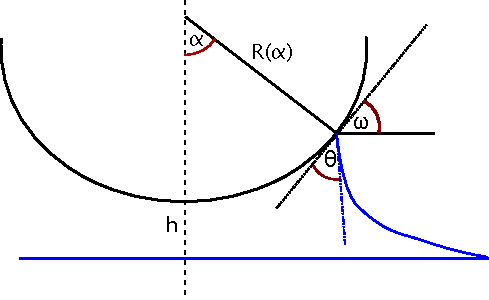
\includegraphics{geometry.pdf}
\end{center}

For a given $(\theta,\alpha)$, the initial coordinates are
\begin{equation}
\left\lbrace
\begin{array}{rcl}
	r_0    & = & R(\alpha) \sin(\alpha)\\
	z_0    & = & (h + R_0) - R(\alpha) \cos(\alpha)\\
	\phi_0 & = & \left(\omega + \theta\right) - \pi\\
\end{array}
\right. 
\end{equation}
where $\omega$ is given by Eq\eqref{eq:omega}.\\

During the simulation, we stop when:
\begin{itemize}
\item $r\leq0$ (which excludes starting at $\alpha=0$)
\item $z\leq0$
\end{itemize}



\end{document}